\chapter{Related Works and Background}
\resetfigpath{relworks_bg}
\glsresetall

\newcounter{algsubstate}
\renewcommand{\thealgsubstate}{\alph{algsubstate}}
\newenvironment{algsubstates}
  {\setcounter{algsubstate}{0}%
   \renewcommand{\State}{%
     \stepcounter{algsubstate}%
     \Statex {\footnotesize\thealgsubstate:}\space}}
  {}

This chapter gives an overview of the vast spectrum of past research related to segmentation in the scenario of sparse supervision.
In particular, we focus on traditional computer vision techniques and
\gls{ml} methods.
Note that in practice, both categories often overlap.

The remaining of this chapter gives some background theory that is relevant to the methods proposed in the remaining of this thesis, namely Random Forest classification and Deep Learning methods.

\section{Related Works}

Past research that address image and volume segmentation using sparse supervision can be roughly divided in two categories,
The first category, mainly focuses on computer vision techniques, while the second focuses on developing Machine Learning techniques.
In practice, both categories often overlap.

We now give an overview of the state-of-the-art in computer vision.
Next, we focus on \gls{ml} methods.


\subsection{Computer Vision Methods}
% Another line of research focuses on the annotation protocol itself so as to complement the above efforts.
% While the most tedious protocol requires that images be manually segmented at a pixel-level, many computer-vision approaches exist to facilitate this task.

Early contributions relied on the Active Contour model \cite{kass88}, which assumes that an initial contour is given and parameterized as the nodes of a spline curve, in this context called an elastic snake.
The segmentation problem is formulated as finding the deformation of the initial snake that minimizes an energy term.
In its simplest form, the energy term is composed of a term that determines the fitting of the snake to the edges of the image, while another term controls the smoothness of the snake.
The energy is then minimized using gradient descent.
Following works alleviate the problem of robustness brought by noisy edge maps by minimizing the Mumford-Shah functional \cite{chan01}, and parameterize the contour using the level-set method \cite{osher88}.

More recently, annotations in the form of scribbles were considered, where the annotator is asked to draw crude delineations of one or several objects of interest, along with a scribble on the background.
A first method that handles such kind of annotations relies on the Random-Walk algorithm \cite{grady06}.
The segmentation problem reduces to assigning to each unlabeled pixel a random-walker. The label of the latter pixel is then determined by finding the label for which the walker has a maximum probability of reaching first.

Relying on the same annotation requirement, the graph-cut approach \cite{boykov2006}
minimizes an Markov Random Field energy objective that considers unary terms (a scalar on each pixel), and a pairwise term that models the similarity of neighboring pixels.
Concretely, the image or volume is represented as a region adjacency graph where each pixel is assigned a node, and edges connect spatially and temporally adjacent pixels.
Each annotated positive pixels is connected to a source node, while annotated negatives are connected to a sink node.
The energy minimization is then performed using the min-cut/max-flow algorithm \cite{goldberg88}.
Using the same algorithm, grab-cut \cite{rother04}, further simplifies the scribble-based annotation protocol by considering bounding-boxes around the object of interest, which provide crude labels on both foreground and background in a single stroke.
An illustration of the graph-cut framework is shown on Fig. \ref{fig:graphcut}, and an example
segmentation on a CT-scan volume is shown on Fig. \ref{fig:graphcut_medical}

\begin{figure}[!h]
  \centering
  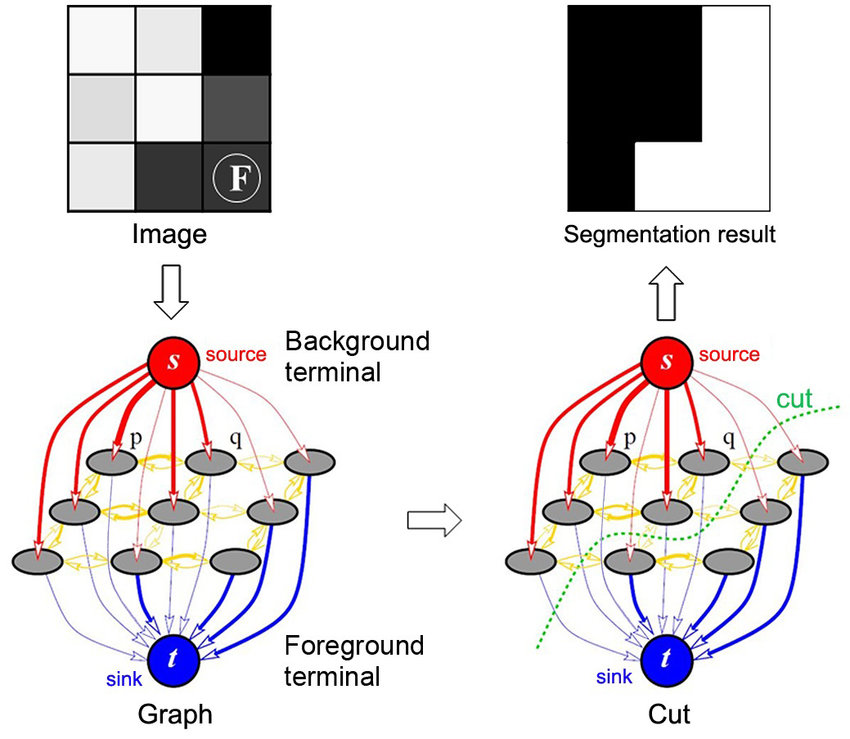
\includegraphics[width=8cm]{graphcut.jpeg}
  \caption{Min-cut/max-flow graph used for graph-cut segmentation. Taken from \cite{xiao17}.}
  \label{fig:graphcut}
\end{figure}

\begin{figure}[!h]
  \centering
  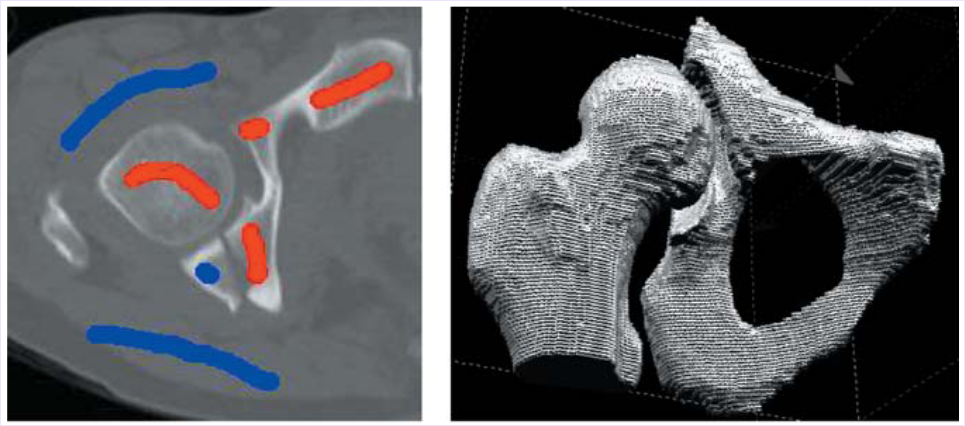
\includegraphics[width=8cm]{graph_cut_med.png}
  \caption{Segmentation of bones in a volumetric CT scan using graph-cut, where the annotator provides
    foreground and background cues from a single slice. (Left) Foreground cues are in red, and
    background cues are in blue. (Right) 3D reconstruction obtained from the slice-wise segmentation.
    Taken from \cite{boykov2006}.}
  \label{fig:graphcut_medical}
\end{figure}

More recently, \cite{krahenbuhl11} proposed an inference strategy to apply a fully-connected \gls{crf} model to coarse pixelwise class-predictions, as a mean to enforce spatial coherence.
Similar to graph-cut, the latter minimizes an energy function that include unary and pairwise potentials, but considers that every pixel is connected to all other pixels.
Fig. \ref{fig:crf} shows examples on natural images.

Closely related to the present thesis, \cite{campbell10, jirik18} endeavors to segment a compact object
present in a volume by means of the graph-cut algorithm, where voxels are connected both spatially and temporally.
Similarly as above, the annotator provides cues to both foreground and background on one or several slices,
and the algorithm performs the propagation throughout the volume.


\subsection{Active Learning and Crowd-sourcing}
The problem of scarcity of labeled data can also be posed in the following manner:
Given a limited annotation budget, i.e. when only a few hours of annotation work can be provided, how can one make the best use of it?

\gls{al} \cite{settles09} considers semi-supervised learning scenarios, where abundant unlabeled data are available.
\gls{al} algorithms aim at selecting the unlabeled samples that are the most informative to the \gls{ml} model.
Conversely, \gls{al} assumes that many unlabeled samples represent redundant information to the late-stage \gls{ml} model.
In \cite{KonSznFua15}, authors devise a strategy to select unlabeled supervoxels of a 3D volume so as to segment volumes of various modalities.
The approach iteratively trains a classifier and takes its entropy as measure of uncertainty.
Combining the latter with a geometric prior, which takes into account intuitive rules on spatial coherence, they sample a batch of most uncertain samples.
The classifier is then re-trained using the newly annotated samples.

Crowd-sourcing, refers to the outsourcing of the annotation task to a high number of annotators \cite{orting19}.
Its use in the frame of medical imaging poses several limitations.
First, the difficulty of the annotation task can prohibit the effective use of crowd-sourcing, e.g when the structure of interest is hard to distinguish \cite{orting19}.
Another limitation is the nature of the data, i.e. one usually prefers to pre-classify brain scans and submit to workers the slices where tumors are present.
Last, one must usually integrate a test-task to ensure the competence of workers, or filter-out annotations provided by ``poorly performing'' workers \cite{park18}.

\subsection{Weakly supervised learning}
An important line of research, weakly supervised learning, endeavors to transpose sparse annotation protocol to the \gls{ml} field.
In \cite{dai15}, authors leverage bounding-box annotations to supervise the training of a \gls{cnn}.
As a follow-up work, \cite{lin16} uses scribbles as annotations.
In \cite{papandreou15}, authors train a \gls{cnn} for semantic segmentation of images by combining pixelwise semantic supervision with image-level supervision in the form of ``tags'' (dog, cat, ...).
Closely related to the present thesis is the work of \cite{bearman16}, who train a \gls{cnn} with a combination of image-level and point-wise supervision.
Concretely, annotations consists in a single 2D location on the object of interest, along with a semantic label corresponding to the class of the object.

A transversal line of research endeavored to combine the traditional graph-cut/\gls{crf} paradigm to \gls{dl} in an attempt to enforce spatial coherence into semantic segmentation models as a refinement step, a requirement that is not immediately achievable through standard loss functions.
The problem is generally formulated as follows: A \gls{dl} predicts the unary potentials, while a late-stage module generates the pairwise potentials and solves the energy objective.
In \cite{rajchl16}, authors leverage the fully-connected \gls{crf} inference procedure of \cite{krahenbuhl11} to segment lung and brain images from bounding-box annotations using a \gls{cnn}.
The \gls{cnn} of \cite{rajchl16} predicts the unary and pairwise potentials and minimize the energy function using a parameterized \gls{crf} using a \gls{rnn}, thereby allowing the parameters of the feature extractor and pairwise similarity model to be optimized in end-to-end fashion.
In \cite{wang18}, authors propose a framework that relies on two steps, where the first generates an initial delineation using a \gls{cnn}, which an annotator can modify manually by drawing scribbles.
Another \gls{cnn} then refines the initial delineation by leveraging the geodesic distance transform \cite{criminisi08}, which combines the initial delineation and the users input.
Their pipeline is shown on Fig. \ref{fig:deepigeos}.

\begin{figure}[!h]
  \centering
  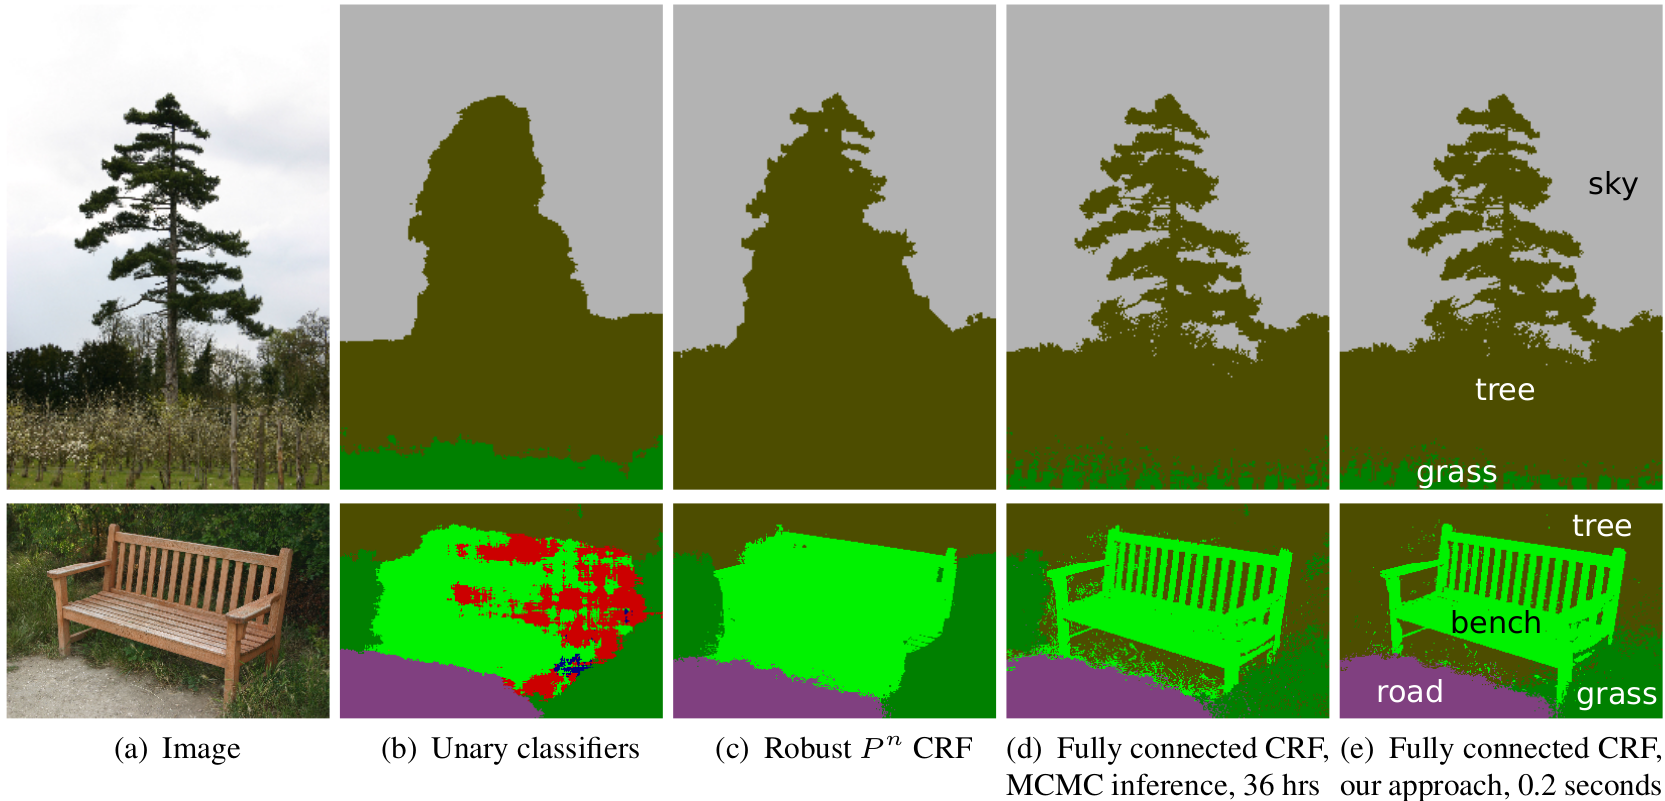
\includegraphics[width=12cm]{crf.png}
  \caption{Example segmentation using CRF on two images. (a) Input image (b) Response of the pixel-wise classifier (unary term) (c) Classification produced by the robust $P^{n}$ CRF \cite{kohli09} (d) Fully-connected CRF using Markov Chain Monte Carlo Inference (e) Approach of \cite{krahenbuhl11}. Taken from \cite{krahenbuhl11}.}
  \label{fig:crf}
\end{figure}

\begin{figure}[!h]
  \centering
  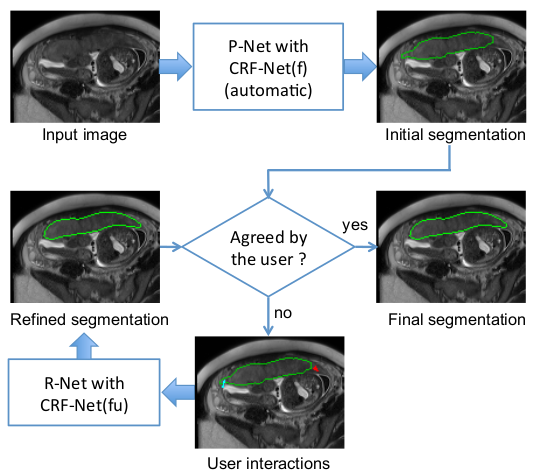
\includegraphics[width=8cm]{deepigeos.png}
  \caption{Deep Interactive Geodesic framework of \cite{wang18}. P-Net proposes an initial automatic segmentation that is refined by R-Net with user interactions indicating mis-segmentations. CRF-Net(f) is a
    back-propagatable CRF that uses free-form pairwise potentials.
    It is extended to be CRF-Net(fu) that employs user interactions as hard constraints. Taken from \cite{wang18}}
  \label{fig:deepigeos}
\end{figure}

Another trend in weakly supervised segmentation is the attention map paradigm.
The latter starts from a standard image-level classification \gls{cnn}, and considers that the response of late layers (before the classification layer), called \gls{cam}, can provide valuable cues on where the network is focusing.
In particular, Grad-CAM \cite{selvaraju17} proposes to generate segmentation maps by combining the activations of late layers with a weighting factor, computed using the backpropagated gradient.
In \cite{li18}, show that such attention maps, as provided by a \gls{cnn} trained only for classification, can be refined using a limited number of pixelwise annotated images.

More recently, adversarial techniques have been employed to semi-supervised semantic segmentation, as a mean to circumvent he computational burden at test time brought by the latter \gls{crf} approach.
In particular, the \gls{gan} approach \cite{goodfellow14} considers a \gls{cnn} that divides in two sub-networks: A generator, and a discriminator.
The first receives a random noise signal which it uses to generate an image that is as ``realistic'' as possible, while the second must distinguish images coming from the generator and real images.
In \cite{luc16}, authors argue that a spatial coherence refinement step similar in spirit to \gls{crf}, can be achieved through the \gls{gan} framework.
In particular, authors combine a standard segmentation network with a discriminator network,
where the latter must distinguish between the predicted label maps of the segmentation network and the groundtruth maps.
Both networks are then trained in parallel using a loss function that combines both objectives.


\subsection{Transfer Learning, Semi-supervised Learning, and Domain Adaptation}
\gls{tl} consists in using a \gls{ml} model trained for the task of interest, but using a training set of different nature than the targeted domain, e.g. train a \gls{cnn} to segment natural objects (trees, cars, ...) for the segmentation of surgical tools.
As pointed out by \cite{oliver18}, an important and implicit assumption in that context is that both datasets share similar data distributions.

\gls{ssl} is a broad category of \gls{ml} algorithm that combines traditional supervised learning tasks, where a scarce fully labeled training dataset is available, along with an abundant unlabeled dataset.
The latter can, under specific conditions, boost the performance of an \gls{ml} model trained with labeled dataset only, i.e. in a fully-supervised manner.
The basic idea is that the ML model may acquire knowledge of the data distribution from the unlabeled set.
Here again, one assumes that both data domains share similar distributions.
In \cite{ghafoorian17}, authors show experimentally that a \gls{nn} trained to segment tumors on MRI brain scans acquired in a given MRI protocol, perform poorly when transferred to another protocol, as the shape, intensities, and contrast level are inconsistent.

\gls{da} addresses the problem of adapting the model so as to take into account domain shift, i.e. the discrepancies between the training and target domain.
In \cite{perone19}, authors devise a strategy to segment MRI scans of spinal cords
using a model trained with images taken at a specific field-of-view, and transfer
to another field-of-view in an unsupervised fashion.
Their approach leverages data-augmentation to enforce a consistency between
the augmented and pristine images of the unlabeled set, while jointly training
with the labeled set with traditional cross-entropy loss.
On the same image modality, \cite{li20} resort to adversarial training. They
jointly train a segmentation model and a discriminator wit shared weights.
The discriminator is trained to discriminate between the source and target domain.

\subsection{Advantages and limitations of existing methods}

The above efforts have provided important solutions to the problem considered in this thesis.
We now wish to provide a summary of their advantages and limitations so as to
justify our contributions, namely our novel annotation protocol and the corresponding
segmentation methods.

While methods based on graph-cut effectively alleviate the annotation burden and proved to be relevant
to the segmentation of volumes and videos, we emphasize here important limitations:

\begin{enumerate}
  \item Both require explicitly (graph-cut) or implicitly (grab-cut) that the annotator provides both
    foreground and background cues so as to define hard constraints and estimate the foreground
    and background unary potentials.
  \item When applied to volumes or videos, the annotation protocol requires that the annotator
    manually select ``relevant'' frames within the volume before providing the cues.
  \item Optimal segmentation results are usually obtained through an iterative process where the annotator
    must examine the segmentation results frame-by-frame and must modify the previous cues to improve the results.
\end{enumerate}

% Next, we note that more recent \gls{dl}-based approaches that aims at combining the graph-cut philosophy
% with the expressivity of \gls{dl} models do not trivially extend to volume and video data.



%%% Local Variables:
%%% mode: latex
%%% TeX-master: "../../main"
%%% End:

\section{Background Theory}

\subsection{Random Forest}
\label{sec:rf}
This section describes the \gls{rf} method, which we will use in the evaluation phase of our deep feature study.
Most of the following content is taken from \cite{hastie09}.

\gls{rf} is an algorithm that builds up from the idea of bootstrap aggregation (bagging).
Bagging consists in combining a commitee of weak learners (high variance and low bias estimators).
Combining such learners allows to decrease the variance one would get when using a single learner.
The \gls{rf} algorithm generates a single decision tree per bootstrap sample.
In the present experimental setup, our task is to predict the class of a given sample (foreground or background).
Once the set of trees are fitted, we infer the class probability of a given sample by computing the average vote over all trees.
The training algorithm is described in Alg. \ref{alg:rf}.

\begin{algorithm}[H]
  \label{alg:rf}
 \caption{Training a Random Forest for classification}
 \begin{algorithmic}[1]
 \Require{Input samples $\bm{X}$, $B$: Number of trees, $N$: Number of samples per tree, $m$: Number of variables to pick at each split, $n_{min}$: Minimum size of a non-leaf node}
  \Ensure{$\bm{T} = \{T_{b}^{i}\}_{i=1}^{N_{T}}$: Set of trees}
    \For{$b \gets 1$ to $B$}
        \State Draw a bootstrap sample $\bm{Z}^{*}$ of size $N$ from $\bm{X}$
        \State Grow a tree $T_{b}$ on $\bm{Z}^{*}$ by recursively repeating the following steps for each non-leaf node of the tree, until the minimum node size $n_{min}$ is reached
        \begin{algsubstates}
                \State Select $m$ variables at random from the $p$ variables
                \State Pick the best variable/split-point among the $m$
                \State Split the node into two children nodes
            \end{algsubstates}
    \EndFor
  \end{algorithmic}
\end{algorithm}


\subsection{Deep Convolutional Neural Network}
\label{sec:cnn}

This chapter serves as an introduction to the basic notions that will come up in the remaining of this thesis, namely the notion of \gls{nn} and \gls{cnn}.
We start by introducing generalities about \gls{nn}.
Most of the content of the present chapter is taken from \cite{goodfellow16}.

\subsubsection{Neural Network}
Deep learning essentially refers to a family of machine learning methods that historically derive from the \gls{mlp}, also known as Neural Network.
An \gls{mlp} aims at approximating an unknown function $f^{*}$ with a function $f(x;\theta)$ parameterized by $\theta$.
More concretely, an \gls{mlp} converts an input $x$ to an output $y$ using a chain of function $f^{(1)} \circ f^{2} \circ \cdots \circ f^{n}(x)$, which justifies its name ``network''.
Each function is usually referred to as ``layer'', while the term ``neural'' comes from the fact that it is originally inspired by neuroscience \cite{mcculloch43}.

As in all machine learning setup, one wants to find the set of parameters $\bm{\theta}$ so as to optimize a cost (or loss) function, for example the \gls{mse}:

\begin{equation}
\mathcal{L}(\bm{\theta}) = \sum_{x\in \mathcal{X}}(f^{*}(x)-f(x;\bm{\theta}))
\end{equation}

One typically use a gradient-descent method to solve the above problem.

In the frame of \gls{mlp}, the functions $f^{m}(x;\bm{\theta_{m}})$ are linear (or fully-connected) layer, i.e. $\bm{\theta}_m=(\bm{w)}_{m},b$, followed by an activation function $\sigma(.)$

\begin{equation}
f^{m}(x;\bm{\theta_{m}}) = \sigma(\bm{x}^{T}\bm{w} + b)
\end{equation}

The activation function, allows to inject non-linearities in the model.
Such function is applied element-wise.
The \gls{relu} is the most widespread.
It writes:

\begin{equation}
\sigma(x) = \max \{0, \bm{x}\}
\end{equation}

\subsubsection{Convolutional Network}
Many machine learning applications relie on structured data, i.e. data that respect a grid-like topology.
Typical examples include time-series and images.
For this reason, \cite{lecun95} introduced the notion of convolutional network, which adapts the previous MLP to leverage the grid-like topolgy in an effective manner.
In particular, the author replaces one or several layers of an MLP with convolutional layers.
In the case of (discrete) images, the convolution operator writes:

\begin{equation}
S(i,j) = (I * K)(i,j) = \sum_{m} \sum_{n} I(m,n) K(i-m, j-n)
\end{equation}

where $I$ is a grayscale image and $K$ is a kernel.
This formulation naturally extends to multi-channel images.
The convolutional operator brings the following advantage over the \gls{mlp}: (1) It naturally leverages the spatial connectivity of pixels.
(2) As the size of the kernel is usually much smaller than the input size (sparse-connectivity), the number of parameters are greatly reduced, which reduces the memory consumption, accelerates the training and improves performances \cite{lecun95}.
Fig. \ref{fig:cnn_con} illustrates the idea of sparse connectivity brought by convolutional layers.

\begin{figure}[!htpb]
  \centering
  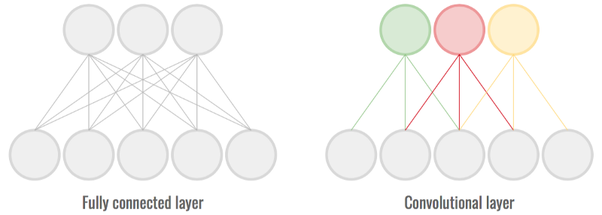
\includegraphics[width=10cm]{fc_vs_conv}
  \caption{(Left) A fully-connected (linear) layer with 1D input at the bottom. (Right) Convolutional layer with a kernel of size 3.}
  \label{fig:cnn_con}
\end{figure}

\subsubsection{Pooling}

Another important component of Convolutional networks are pooling layers, which allow to increase the receptive field of the convolutional operators as the depth is increased.
This effectively allow to capture, in the case of images, visual features at different spatial scales, i.e. that gets more global as the depth increases.
In particular, the max-pooling operator computes for each spatial location the maximal filter response over a pre-defined neighborhood (see fig. \ref{fig:max_pool})

\begin{figure}[!htpb]
  \centering
  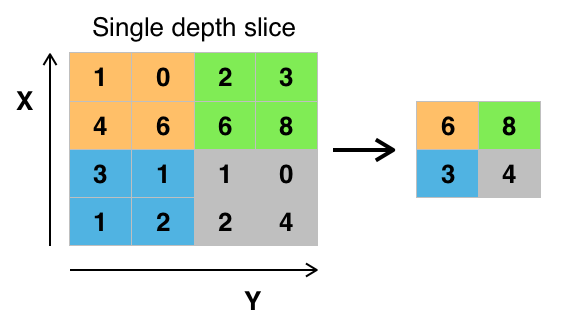
\includegraphics[width=10cm]{max_pooling}
  \caption{(Left) Input. (Right) Output of max-pooling layer. Each color represents a set of values included in the sliding window.}
  \label{fig:max_pool}
\end{figure}
Figure \ref{fig:cnn} illustrates a CNN applied to an image processing task.

\subsubsection{Optimization}
Since the advent of deep learning, many optimization algorithms have been proposed and proved to be effective, each with their own pros and cons.
To name a few: \gls{sgd}, Adam \cite{kingma14}, and RMSProp \cite{tieleman12}.
As the two latter are essentially improvements of \gls{sgd}, we restrict this section to \gls{sgd} (see \ref{alg:sgd}).
In practice, effectively training a deep learning model demands careful study of hyper-parameters.
The most crucial is certainly the learning rate $\lambda$ which controls the fraction of gradient-estimate one wants to use to update $\bm{\theta}$.
Also, one needs to initialize $\bm{\theta}$ to random values.
The latter step has been an important object of study, e.g \cite{he15}, \cite{glorot10}.

\begin{algorithm}[H]
  \label{alg:sgd}
 \caption{Stochastic Gradient Descent (SGD)}

 \begin{algorithmic}[1]
  \Require{Training data ${(\bm{x}_{i},y_{j})}_{i=1}^{N}$, learning rate $\lambda$, initial parameters $\bm{\theta}$}
  \Ensure{Model parameters $\bm{\theta}$}
  \Repeat
    \State Sample a minibatch of m examples from the training set $\{(\bm{x}_{1},y_{1}), \cdots, (\bm{x}_{m},y_{m})\}$
    \State Compute gradient estimate: $\hat{\bm{g}} \leftarrow + \frac{1}{m} \nabla_{\bm{\theta}}\sum_{i}\mathcal{L}(f(\bm{x}_{i}; \bm{\theta}), y_{i})$
    \State Apply gradient update: $\bm{\theta} \leftarrow \bm{\theta} - \lambda \hat{\bm{g}}$
    \Until {stopping criterion is met}
  \end{algorithmic}
\end{algorithm}


\subsubsection{Batch normalization}
As already mentioned, training a CNN demands a careful tuning of the learning rate in order to converge to a proper solution.
Practical issues such as exploding/vanishing gradient arise when the latter is two high/low, respectively.
In particular, as noted in \cite{ioffe15}, the input distribution of a given layer is dependent on the parameters of all preceding layers, a phenomenon called internal covariate shift.
To circumvent the latter problem, a batch normalization can be added at the output of each layer to normalize the values of a given minibatch to a normal distribution.
Additionally, such normalization often needs to combine with an activation function, and therefore will have its left tail zeroed-out in the case of a \gls{relu}.
To circumvent that, authors add learnable scaling and shifting parameters, $\gamma$ and $\beta$, respectively.
Also, batch normalization also has a regularization effect due to fluctuations in mini-batch statistics \cite{gastaldi17}.
The algorithm is described in alg. \ref{alg:batchnorm}.

\begin{algorithm}[H]
  \label{alg:batchnorm}
 \caption{Batch Normalization}
 \begin{algorithmic}[1]
  \Require{Minibatch of size $M$: $\mathcal{B}=\{(\bm{x}_{i})\}_{i=1}^{M}$, learnable scaling and shifting parameters, $\gamma$ and $\beta$}
  \Ensure{$\bm{x}'_{i}=\text{BN}(\bm{x}_{i};\gamma,\beta)$}
    \State Compute mean: $\mu_{\mathcal{B}}\leftarrow \frac{1}{m}\sum_{i=1}^{M}\bm{x}_{i}$

    \State Compute variance: $\sigma^{2}_{\mathcal{B}}\leftarrow \frac{1}{m}\sum_{i=1}^{M}(\bm{x}_{i}-\mu_{\mathcal{B}})$

    \State Normalize: $\hat{\bm{x}}_{i}\leftarrow \frac{\bm{x}_{i}-\mu_{\mathcal{B}}}{\sqrt{\sigma^{2}_{\mathcal{B}} + \epsilon}}$

    \State Scale and shift: $x_{i}'\leftarrow \gamma \hat{\bm{x}}_{i} + \beta \equiv \text{BN}(\bm{x}_{i};\gamma,\beta)$

 \end{algorithmic}
\end{algorithm}

\begin{figure}[!htpb]
  \centering
  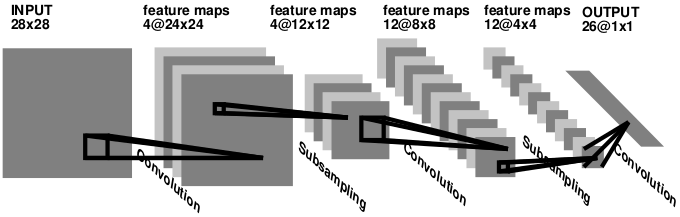
\includegraphics[width=13cm]{cnn}
  \caption{Convolutional Neural Network applied to an image task.
    The network applies a succession of convolution, and pooling (subsampling) operation.
  Activation functions are not represented. Figure taken from \cite{lecun95}}
  \label{fig:cnn}
\end{figure}

\subsubsection{Convolutional Autoencoder}
The basic idea of \gls{ae}, first introduced in \cite{vincent10}, consists in training a model in an unsupervised manner, so as to generate a compressed representation of the input.
Such compressed representation, often called feature vector, is typically used in a subsequent machine learning task.
In particular, an \gls{ae} is composed of two modules: An encoding function $f_{\theta}$, and a decoding function $g_{\phi}$.
The training objective is to minimize the discrepancy between an input sample $x$ and its reconstructed version $x'$.
An example is shown on Fig. \ref{fig:ae}.

For example, using the \gls{mse} criterion, one writes:

\begin{equation}
\mathcal{L}_{AE} = \mathbb{E}_{x_{i}}||f_{\theta}(g_{\phi}(x)) - x ||
\end{equation}


\begin{figure}[!htpb]
  \centering
  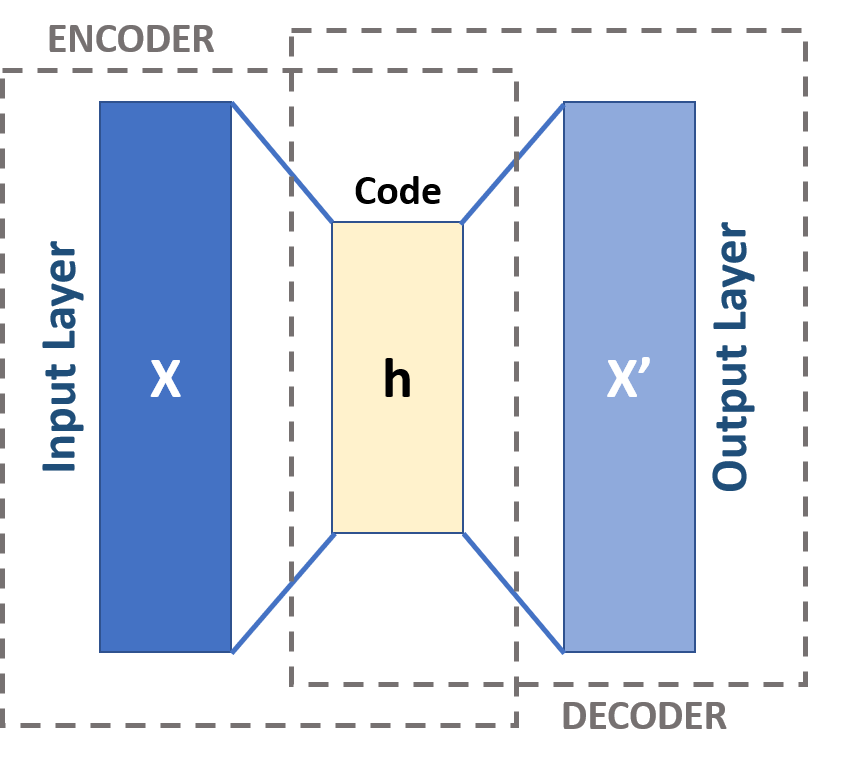
\includegraphics[width=7cm]{ae}
  \caption{Convolutional Autoencoder.
    The input sample $x$ passes through an encoder.
    The output of the encoder, called $h$, passes through a decoder to give the reconstructed version $x'$.
    In yellow is the bottleneck.}
  \label{fig:ae}
\end{figure}

\section{Multi-path tracking}
This section gives a theoretical background to the multi-path tracking problem, as first developed in \cite{berclaz11}.
The latter framework is leveraged in our first major contribution, where we perform tracking of over-segmented regions accross a sequence, where each region can be part of object of interest.

We develop our multi-path tracking framework through the following steps.
(1) We first represent our sequence as a stack of occupancy grid, where each element of a grid represent an over-segmented region.
The elements of these grids are then represented as the nodes of a directed acyclic graph, connected by edges that represent admissible motions.
(2) We introduce the notion of discrete flow variables, which represent the number of objects passing from one position of the grid to another.
(3) We formulate the multi-path tracking problem as a \gls{map} problem, where the grid occupancies are binary random variables.
(4) We show how the latter problem, under the Markov assumption, is identical to an \gls{ip}.
(5) As the latter is NP hard, we show that relaxing it to a continuous \gls{lp} and solving it using off-the-shelf solvers converges to the optimal solution.
(6) We further show that the implicit spatio-temporal relations of our occupancy grid allow to leverage the \gls{ksp} algorithm.

Formally, we start by formulating our problem in the network-flow paradigm.
Next, we show the latter allow to solve a \gls{map} problem, where the objectness of over-segmented regions are the variables to optimize, and show how the likelihoods can be modeled by appearance similarity models.
Last, we show how solving the latter \gls{map}, when cast into a network flow problem, can be solved efficiently.

\subsection{Segmentation as a network flow problem on over-segmented regions}
We depart from the work of \cite{berclaz11} on two aspects: (1) In contrast to the latter authors, who represent a sequence as a stack of coarse grids, i.e. each cell represent a physical position and the relative locations are fixed in advance, we rather consider that our sequence is over-segmented into superpixels.
(2) We leverage the ``tracklet'' paradigm, where each over-segmented region is represented as a short track in which flow is allowed to pass through.


In particular, we generate on each frame, indexed by a time variable $t$, a set of $N_{t}$ non-overlapping over-segmented regions $\mathcal{S}_{t}=\{s_{t}^{n}\}_{n=1}^{N_{t}}$.
Within the directed graph representation, we represent each over-segmented region $s^{t}_{n}$ by a couple of nodes connected by a \textit{visiting} edge $e^{n}_{t}$.
As a sidenote, the latter is often refered to as a ``tracklet'' \cite{zhang08}.
So as to allow objects to transit from one frame to the next, we add \textit{transition} edges $e^{(n,m)}_{t}$ that connect region $s^{n}_{t}$ to region $s^{m}_{t+1}$.
Each edge is labeled with a discrete non-negative flow variable.
In particular, $f_{t}^{n}$ corresponds to the flow transiting through edge $e_{t}^{n}$, while $f_{t}^{n,m}$ corresponds to the flow passing from region $s_{t}^{n}$ to region $s_{t+1}^{m}$.
Next, we impose conservation of flow, which imposes that the quantity of flow that passes into a visiting edge is equal to the quantity of flow that leaves it. Formally:

\begin{equation}
  \label{eq:flow_conserv}
  \forall t,n \quad f_{t}^{n} = \sum_{n:m\in \mathcal{N}(n)}f_{t}^{n,m}
\end{equation}

When $\mathcal{N}(n)$ is a spatial neighborhood centered on region $n$ that defines admissible motion.

Next, as we assume that each region can contain a maximum of one object. Formally:

\begin{equation}
  \label{eq:capa_constrain}
  \forall t,n \quad f_{t}^{n} \leq 1
\end{equation}

Note that Eq. \ref{eq:flow_conserv} and \ref{eq:capa_constrain} implictly enforce a maximum flow constraints on transition edges.

At the root of our segmentation framework lies the basic idea that our object to segment is composed of over-segmented regions that are spatially and temporally organized.
Moreover, we expect that the size of our object of interest changes through time/slice, e.g. a brain tumor on transversal slices appears to grow and shrink again as one scrolls from one end of the scan to the other end.
To address this requirement, we introduce two kinds of \textit{virtual} nodes: A source node and a sink node.
The first acts like a tap, i.e. it pushes flow inside the graph and increases the total mass, while the second allows to evacuate mass.
We ensure a flow-mass conservation through the constraint:

\begin{equation}
  \label{eq:mass_constrain}
  \sum_{t,m\in \mathcal{N}(\xi_{t})}f_{xi_{t},m} = \sum_{k:\mathcal{X}\in\mathcal{N}(k)}f^{t}_{k,\mathcal{X}}
\end{equation}

Where the $\xi_{t}$ are proxy source nodes that allow pushing flow on frame $t$, and $\mathcal{X}$ is the sink node.
Fig. \ref{fig:flownetwork} illustrates our network flow.

\begin{figure}[!htpb]
  \centering
  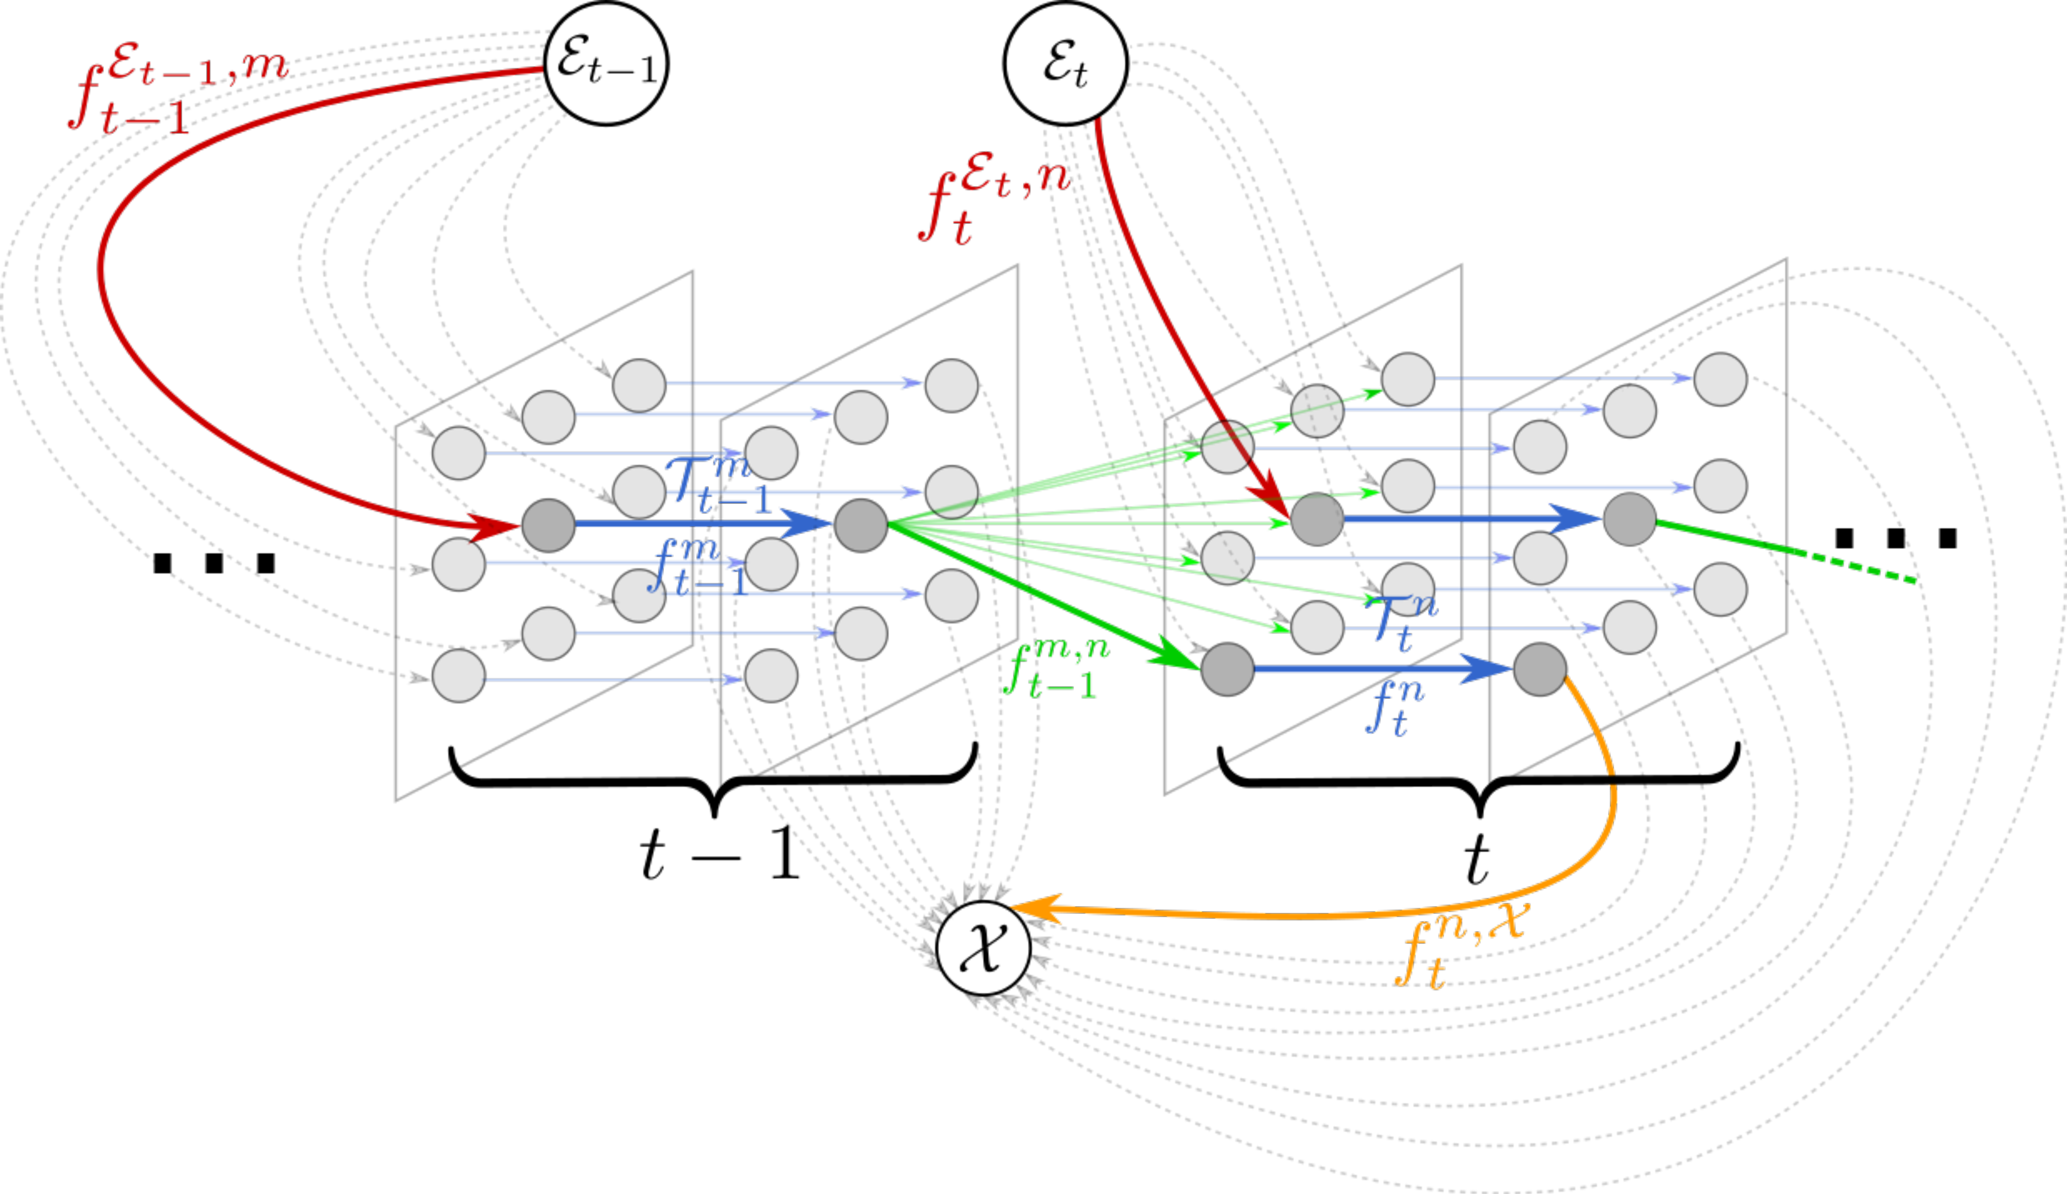
\includegraphics[width=13cm]{network}
  \caption{Illustration of our flow network. Each over-segmented region is assigned a visiting edge (in blue).
    Flow is allowed to pass from one frame to the next through the transition edges (in green).
    A set of proxy source nodes $\xi_{t}$ allow to push flow into the network through entrance edges (in red).
  The sink node $\mathcal{X}$ allows to evacuate flow through exit edges (in orange).}
  \label{fig:flownetwork}
\end{figure}

\subsection{Maximum a Posteriori formulation}
We first formulate an \gls{map} estimation problem, where the random variable to optimize for denotes the presence of objects at discrete time-space locations.
Next, we emphasize how the network flow paradigm developed above is leveraged in order to solve the \gls{map} estimation problem.

Let $\bm{Y}={Y^{n}_{t}|\forall(t,n)}$ a set of binary random variable that take value $1$ when region $s^{n}_{t}$ is object, and $0$ otherwise, while $\bm{I}_{t=1}^{N}$ and $\bm{g}_{t=1}^{N}$ are a set of $N$ images and user-provided 2D locations, respectively.
We define our segmentation task as.

\begin{equation}
  \label{eq:map}
  y^{*} = \arg \max_{y \in \mathcal{Y}}P(\bm{Y}=\bm{y}|\bm{I}, \bm{g})
\end{equation}

where $y^{*}$ are the optimal binary labels.
Assuming that $Y^{t}_{n}$ is conditionally independent given the observed variables, we rewrite Eq. \ref{eq:map} as

\begin{equation}
  \label{eq:bg_map2}
  y^{*} = \arg \max_{y \in \mathcal{Y}}\prod_{i,j,t} P_{visit}(Y^{t}_{n}|\bm{I}, \bm{g}) P_{trans}(Y^{t}_{n}|I^{t-1},\bm{g}) P_{in}(Y^{t}_{n}|I^{t},\bm{g})
\end{equation}

The decomposition of \ref{eq:bg_map2} shows three different likelihood models that will provide the costs of blue, red, and green edges of Fig. \ref{fig:flownetwork}, respectively.
Next, we want to convert Eq. \ref{eq:bg_map2} to a linear sum of its random variables.
To this end, we provide the following lemma:

\begin{lemma}
  \label{lm:linprog}
  Let $y^{*}=\arg\max_{y\in\mathcal{Y}}P(Y^{t}_{n}|\bm{x})$ an \gls{map} problem to solve, and $\rho^{t}_{n}=P(Y^{t}_{n}=1|\bm{x})$ the marginal posterior probability that $Y^{t}_{n}$ contains an object.
  The latter \gls{map} problem can be rewritten as a linear expression of the binary random variables through:

  \begin{align}
    y^{*} &= \arg \max_{y\in\mathcal{Y}} \quad \log \prod_{t,n} P(Y^{t}_{n}=y^{t}_{n}|\bm{x})\\
          &= \arg \max_{y\in\mathcal{Y}} \sum_{t,n} \log P(Y^{t}_{n}=y^{t}_{n}|\bm{x}) \\
    &= \arg \max_{y\in\mathcal{Y}} \sum_{t,n} (1-y^{t}_{n})\log P(Y^{t}_{n}=0|\bm{x}) + y^{t}_{n}\log P(Y^{t}_{n}=1|\bm{x}) \label{eq:lmbinary}\\
    &= \arg \max_{y\in\mathcal{Y}} \sum_{t,n} y^{t}_{n}\log \frac{P(Y^{t}_{n}=1|\bm{x})}{P(Y^{t}_{n}=0|\bm{x})} \label{eq:lmignore}\\
    &= \arg \max_{y\in\mathcal{Y}} \sum_{t,n} y^{t}_{n}\log \frac{\rho^{t}_{n}}{1-\rho^{t}_{n}}
  \end{align}

Where Eq. \ref{eq:lmbinary} is true because of the binarity of the random variables, and Eq. \ref{eq:lmignore} is obtained by ignoring a term independent on $\bm{y}$.
\end{lemma}

\subsection{Linear Programming Formulation}
Our original \gls{map} problem of Eq. \ref{eq:map} can now be rewritten as an \gls{ip} thanks to lemma \ref{lm:linprog}.
In particular, we let our binary random variables $y^{t}_{n}=1$ when the flow variables $f^{t}_{n}=1$, and $0$ otherwise.
Our \gls{ip} writes:

\begin{subequations}
\label{eq:bg_int_prog}
\begin{align}
\intertext{Maximize}
&\sum_{t,n} \log{\frac{\rho_n^t}{1-\rho_n^t}}f_n^t + \sum_{t,m} \log{\frac{\alpha_{m,n}^{t}}{1-\alpha_{m,n}^{t}}}\sum_{t,n}f_{m,n}^{t} + \sum_{t,n} \log{\frac{\beta_n^t}{1-\beta_n^t}}f_{\mathcal{E}_t,n}^{t},\label{eq:bg_loglikelihood}\\
\intertext{subject to,}
&f_{m,n}^{t} \geq 0, \qquad \forall t,m,n \label{eq:nonneg_flow}\\
&\sum\limits_{n}f_{m,n}^{t} \leq 1, \qquad \forall t,m,n \label{eq:bg_cap1_trans}\\
&\sum_m f_{m,n}^{t} - \sum_p f^{t-1}_{p,m} \leq 0, \qquad \forall t,m,n,p \label{eq:bg_conserv1}\\
&\sum_{m,t} f^t_{\mathcal{E}_t,m} - \sum_p f_{p,\mathcal{X}} \leq 0, \qquad \forall t,m\label{eq:bg_conserv2}
\end{align}
\end{subequations}

As mentioned in \cite{berclaz11}, the above \gls{ip} is NP-complete, which prohibits the use of off-the-shelf \gls{lp} solvers.
To circumvent that, authors suggest to relax the \gls{ip} into an \gls{lp}.
In particular, the problem of Eq. \ref{eq:bg_int_prog} is converted to its \textit{canonical form}, by aggregating Eq. \ref{eq:bg_cap1_trans}, \ref{eq:bg_conserv1}, and \ref{eq:bg_conserv2} into a constraint matrix $C$ such that

\begin{equation}
  C \cdot \bm{f} \leq [1, \ldots, 1, 0, \ldots, 0]^{T}
\end{equation}
Thanks to the  \textit{total unimodularity} of the constraint matrix, the \gls{lp} converges to integer solutions.
We kindly redirect the reader to the proof given in \cite{berclaz11}.

\section{Recursive Bayesian Parameter Estimation}
In this section, we provide a theoretical background to recursive bayesian parameter estimation as a complement to our last contribution.
In particular, this contribution relies on estimating class-priors on every frame of a sequence, i.e. estimating the proportion of positive over-segmented regions.

Here, we start by formulating the state-estimation problem using the hidden Markov model framework.
Next, we show how the traditional Kalman filtering algorithm \cite{kalman1960} allows to estimate a posteriori state-estimates using observations in an efficient manner when specific assumptions are validated.
We then elaborate on the \gls{ekf} and its successor, the \gls{ukf}

\subsection{Hidden Markov model}
In recursive bayesian parameter estimation, we aim at estimating the true value of a state variable $\bm{x}$ over time, by leveraging incoming noisy observations $\bm{z}$.
We assume that a mathematical model exists that evolve the current true value of the state to the state at the previous time-step.
Furthermore, another model provides the relation between the observation of and the state.
Formally, we define the following discrete-time dynamic system:

\begin{align}
  \bm{x}_{k+1}&=F(\bm{x}_{k},\bm{v}_{k}) \label{eq:bg_state_trans}\\
  \bm{z}_{k}&= H(\bm{x}_{k}, \bm{n}_{k}) \label{eq:bg_proc}
\end{align}

where $\bm{x}$ denotes the state variable, $\bm{z}$ denotes the observations,
$F$ and $H$ are the transition and process models, respectively, while $\bm{v}$ and $\bm{n}$ are the process and transition noise, respectively.
Fig. \ref{fig:hmm} represents the dynamic system of Eq. \ref{eq:bg_state_trans} and \ref{eq:bg_proc} as a directed graph, where edges represent probabilistic relationships.
In the recursive bayesian filtering paradigm, we assume that all variables are stochastic.
Furthermore, the systems follows the Markov assumption, i.e. every variable is conditionally independent of its nondescendents, given its parents \cite{geiger90}.
Formally,

\begin{align}
  p(\bm{x}_{k+1}|\bm{x}_{k}, \bm{x}_{k-1},\ldots,\bm{x}_{0})=p(\bm{x}_{k+1}|\bm{x}_{k})\\
  p(\bm{z}_{k}|\bm{x}_{k}, \bm{x}_{k-1},\ldots,\bm{x}_{0})=p(\bm{z}_{k}|\bm{x}_{k})
\end{align}

When the state variables are unobserved, but is dependent on another observable process, we call such a system a \gls{hmm}.

\begin{figure}[!htpb]
  \centering
  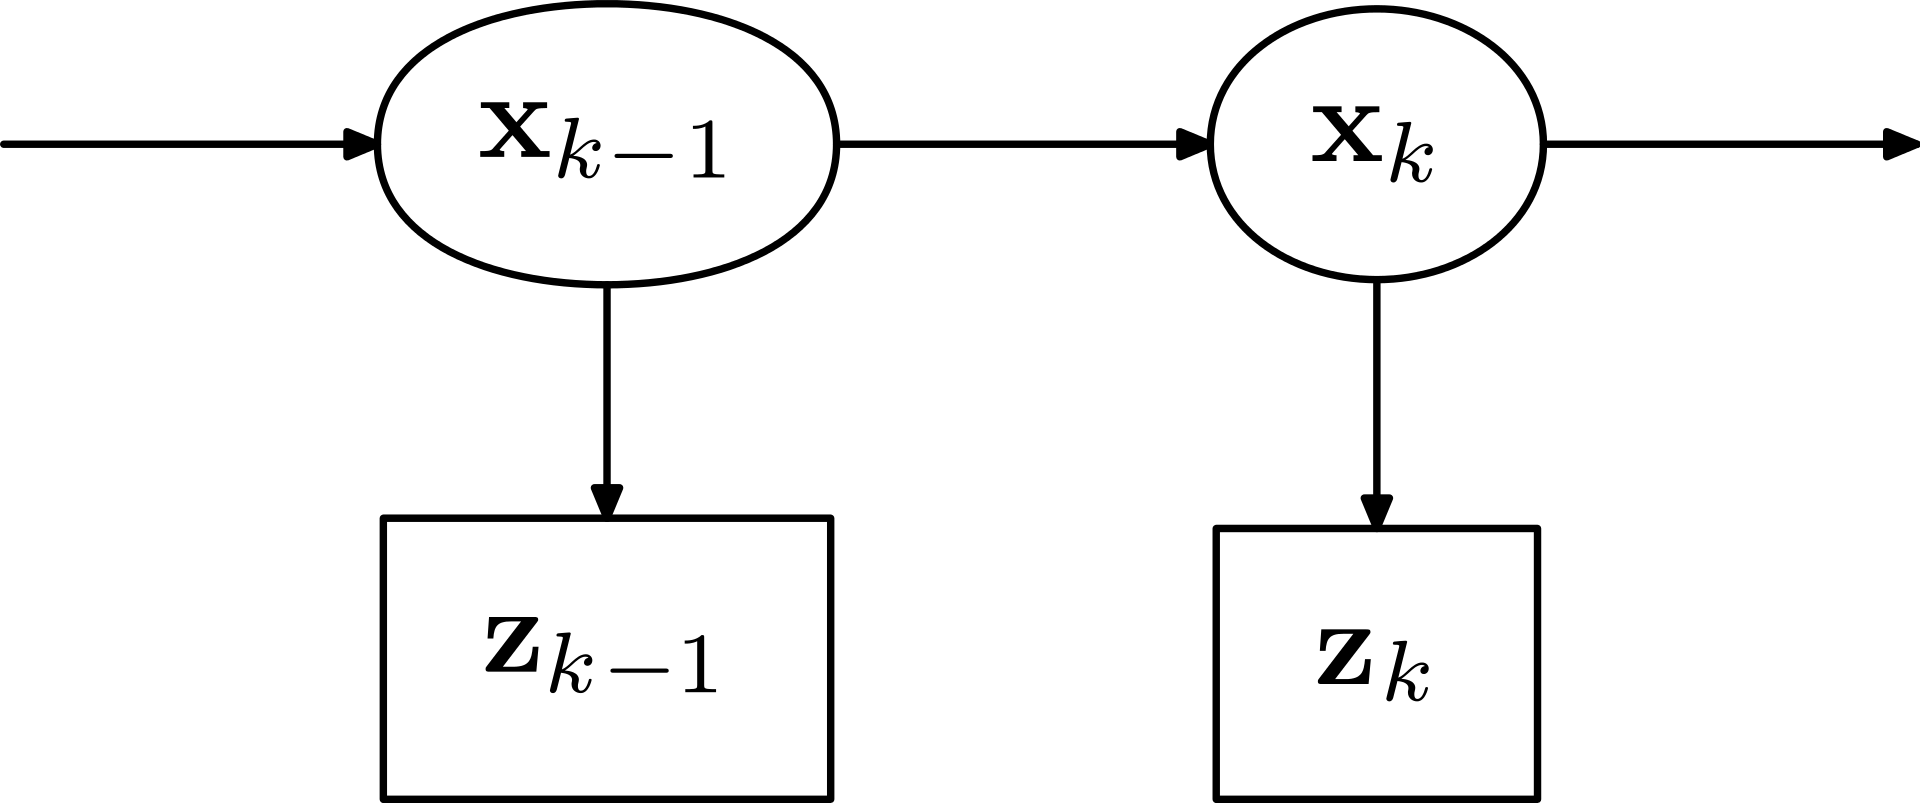
\includegraphics[width=10cm]{hmm}
  \caption{Graphical representation of a \gls{hmm}. $x$ are the hidden variables, while $z$ are the observations.
  Edges represent probabilistic relationships.}
  \label{fig:hmm}
\end{figure}

\subsection{Recursive bayesian filtering and Kalman Filter Equations}
In recursive bayesian filtering, we are interested in estimating the \gls{pdf} of the current state using the history of observations up to the current time-step, written $p(\bm{x}_{k}|\bm{z}_{0:k}$, where $\bm{z}_{0:k}$ is a short form for $\bm{z}_{0},\ldots, \bm{z}_{k}$.

Using Baye's rule, we rewrite:
\begin{equation}
  \label{eq:bg_aposteriori}
  p(\bm{x}_{k}|\bm{z}_{0:k}) = \frac{p(\bm{x}_{k}|\bm{z}_{0:k-1})\cdot p(\bm{x}_{k}|\bm{z}_{k})}{p(\bm{x}_{k}|\bm{z}_{0:k-1})}
\end{equation}

The left term of the denominator of Eq. \ref{eq:bg_aposteriori} is called the a-priori probability distribution of the current state.
We rewrite it in a recursive form as
\begin{equation}
  \label{eq:bg_prior}
  p(\bm{x}_{k}|\bm{z}_{0:k-1}) = \int p(\bm{x}_{k}|\bm{x}_{k-1}) \cdot p(\bm{x}_{k-1}|\bm{z}_{0:k-1}) d\bm{x}_{k-1}
\end{equation}

Next, the denominator is a normalization term written:
\begin{equation}
  \label{eq:bg_norm_cst}
  p(\bm{z}_{k}|\bm{z}_{0:k-1}) = \int p(\bm{x}_{k}|\bm{z}_{0:k-1}) \cdot p(\bm{z}_{k}|\bm{x}_{k}) d\bm{x}_{k}
\end{equation}

In this general form, the exact inference of Eq. \ref{eq:bg_aposteriori} is untracktable.
However, many algorithms exists that solve this problems approximately under specific conditions, e.g. Expectation-Maximization \cite{dempster77} and Markov-chain Monte Carlo \cite{geyer92}.

\subsubsection{Kalman Filter}

Under the more restrictive assumptions that (1) models $F$ and $G$ are linear functions, (2) the initial values of the state variables follow a multivariate normal distribution, and (3) the process and observation noise are additive, zero-mean and normally distributed, the \gls{KF} algorithm provides exact solutions.
This comes from the fact that under the above conditions, the a-posteriori pdf \ref{eq:bg_aposteriori} is also normally distributed, and is therefore fully characterized by its first and second moment, i.e. its mean and covariance.
Under these conditions, the condition \gls{pdf} is fully characterized by its first and second moment, i.e. mean and covariance.

the \gls{kf} only needs to propagate the
Under these assumptions, the state-space model is rewritten :

\begin{align}
  \bm{x}_{k+1}&=F_{k}\bm{x}_{k} B_{k}u_{k} + \bm{v}_{k} \label{eq:bg_state_trans_kf}\\
  \bm{z}_{k}&= H_{k}\bm{x}_{k} + \bm{n}_{k} \label{eq:bg_proc_kf} \\
  \bm{x}_{0}&= \bm{\bar{x}}_{0} + \mathcal{N}(0,S) \label{eq:bg_init_kf}
\end{align}

Where $\bm{v}_{k}=\mathcal{N}(0,Q)$, $\bm{n}_{k}=\mathcal{N}(0,R)$ are the process and observation noise signals, respectively, while $Q$, $R$, and $S$ are the process, observation and initial covariance matrices, respectively.

\subsubsection{Kalman Filter inference}
We now provide an overview of the main steps of the \gls{kf} algorithm.
For the detailed derivations, we refer the reader to \cite{thacker98}.

The problem of \gls{kf} is to produce an optimal estimate of the hidden state variable, written $\bm{\hat x}_{k}$, given the observations.
In particular, it takes as criteria of optimality the \gls{mse} between the estimate and the true value of the state.
As shown in \cite{ribeiro04}, the estimator that minimizes this criteria is the the conditional mean, i.e.

\begin{equation}
  \label{eq:bg_cond_mean}
  \bm{\hat x}_{k} = \mathbb{E}[\bm{x}_{k}|\bm{z}_{0:k}]
\end{equation}

The inference is decomposed into a prediction and filtering step, i.e.

\begin{itemize}
    \item \textbf{Prediction: } $p(\bm{x}_{k}|\bm{z}_{0:k}) \rightarrow p(\bm{x}_{k+1}|\bm{z}_{0:k})$
    \item \textbf{filtering: } $p(\bm{x}_{k+1}|\bm{z}_{0:k}) \rightarrow p(\bm{x}_{k+1}|\bm{z}_{0:k+1})$
\end{itemize}

Where the prediction step applies the transition function to the current state estimate, thereby computing the a-priori conditional \gls{pdf}, and the filtering corrects the latter using the newly arrived observation $\bm{z}_{k+1}$, thereby computing the a-posteriori conditional \gls{pdf}.

Formally, the prediction step resolves to the following recursive equation:

\textbf{Prediction:}
\begin{align}
  \bm{\hat x}^{-}_{k+1}&=F_{k} \bm{\hat x}_{k} + B_{k}u_{k} \label{eq:bg_apriori_estim}\\
  P_{k+1}^{-}&=F_{k} P_{k} F_{k}^{T} + Q_{k} \label{eq:bg_apriori_cov}
\end{align}

Where $P_{k}$ is the covariance matrix of the state, and $\bm{\hat x}^{-}$ denotes the a-priori state estimate.
Eq. \ref{eq:bg_apriori_estim} computes the a-priori state estimate, and Eq. \ref{eq:bg_apriori_cov} computes the a-priori state covariance.

\textbf{Correction:}
\begin{align}
  \bm{\tilde y}_{k+1} &= \bm{z}_{k+1} - H_{k+1} \bm{\hat x}_{k+1}^{-} \label{eq:bg_innov} \\
  T_{k+1} &= H_{k+1} P_{k+1}^{-} H_{k+1}^{T} + R_{k} \label{eq:bg_innov_cov} \\
  K_{k+1} &= P_{k+1}^{-} H_{k+1}^{T} T_{k+1}^{T} \label{eq:bg_kf_gain}\\
  \bm{\hat x}_{k+1} &= \bm{\hat x}_{k+1} + K_{k} \bm{\tilde y}_{k+1} \label{eq:bg_aposteriori_state_estim}\\
  P_{k+1} &= (I - K_{k+1}H_{k+1}) P_{k+1}^{-} \label{eq:bg_aposteriori_cov_estim}
\end{align}

Eq. \cref{eq:bg_innov,eq:bg_innov_cov,eq:bg_kf_gain,eq:bg_aposteriori_state_estim,eq:bg_aposteriori_cov_estim} compute the state innovation, covariance innovation, Kalman gain, a-posteriori state estimate, and a-posteriori covariance estimate, respectively.
In practice, the two above steps are applied each time a new observation arrives.

\subsection{Unscented Kalman Filter}
The standard \gls{kf} framework allows to compute the a-priori state estimate, Kalman gain, and a-posteriori state estimate \textit{exactly}, by propagating the mean and covariance of the state, two quantities that fully characterize its \gls{pdf}, through the linear-system dynamics.
However, when the system is non-linear, the \gls{kf} is prohibited, since the a-priori and a-posteriori conditional \gls{pdf}, after transformation, become non-gaussian.
The \gls{ekf} \cite{ribeiro04} attempts to generalize \gls{kf} to such scenario by approximating the moments of these \gls{pdf} using first-order Taylor expansion around the current estimates.
We choose not to delve into the details of \gls{ekf}, and simply mention that the latter approximation, in practice, bring sub-optimal results and often lead to the divergence of the filter \cite{wan00}.

We now give an overview of the \gls{ukf}, which attempts to amend the flaws of \gls{ekf}.

\subsubsection{Unscented Transformation}
\gls{ukf} considers the \gls{ut} \cite{julier96}, which discretize a (continuous) \gls{pdf} into a set of carefully chosen points so as to (1) capture the true mean and covariance accurately, and (2) capture the true posterior statistics up to the third order after propagation through non-linear functions.
This approach departs from \gls{ekf} in that, the non-linear functions are applied to these transformed points directly.

In particular, let $\bm{x}$ a \gls{grv} of dimension $L$ with mean $\bm{\bar x}$ and covariance $P_{x} \in \mathbb{R}^{L \cdot L}$.
Next, let $\bm{\mathcal{X}}$ a matrix whose rows contain $2L+1$ sigma-vectors $\bm{\mathcal{X}}_{i}$, and $\mathcal{Y} = g(\mathcal{X})$ its transformation trough an arbitrary function $g$.
The procedure is \cite{wan00}:
\begin{enumerate}
  \item Compute sigma-points $\mathcal{X}$ and corresponding weight matrix $W$ as:
    \begin{itemize}
      \item $\mathcal{\bm{X}}_{0} = \bm{\bar x}$
      \item $\mathcal{\bm{X}}_{i} = \bm{\bar x} + (\sqrt{(L + \lambda) P_{x}})_{i} \quad i=1,\ldots,L$
      \item $\mathcal{\bm{X}}_{i} = \bm{\bar x} - (\sqrt{(L + \lambda) P_{x}})_{i} \quad i=L+1,\ldots,2L+1$
      \item $W_{0}^{(m)}=\lambda / (L + \lambda)$
      \item $W_{0}^{(c)}=\lambda / (L + \lambda) + (3 - \alpha^{2})$
      \item $W_{i}^{(m)}=W_{i}^{(c)}= 1 / [2(L + \lambda)]$
    \end{itemize}
\end{enumerate}

Where $\lambda = L (\alpha^{2}-1)$ is a scaling parameter, and $\alpha$ determines the spread of sigma points around the mean.
Next, the sigma-points are propagated through $g$:
\begin{equation}
  \mathcal{Y}_{i} = g(\mathcal{X}_{i}) \quad i=0,\ldots,L
\end{equation}
Finally, we obtain the statistics of the output through the following approximations:
\begin{align}
  \bm{\bar y} & \approx \sum_{i=0}^{2L} W_{i}^{(m)}\mathcal{Y}_{i} \\
  P_{y} & \approx \sum_{i=0}^{2L} W_{i}^{(c)}[\mathcal{Y}_{i}-\bm{\bar y}][\mathcal{Y}_{i}-\bm{\bar y}]^{T}
\end{align}

\begin{figure}[!htpb]
  \centering
  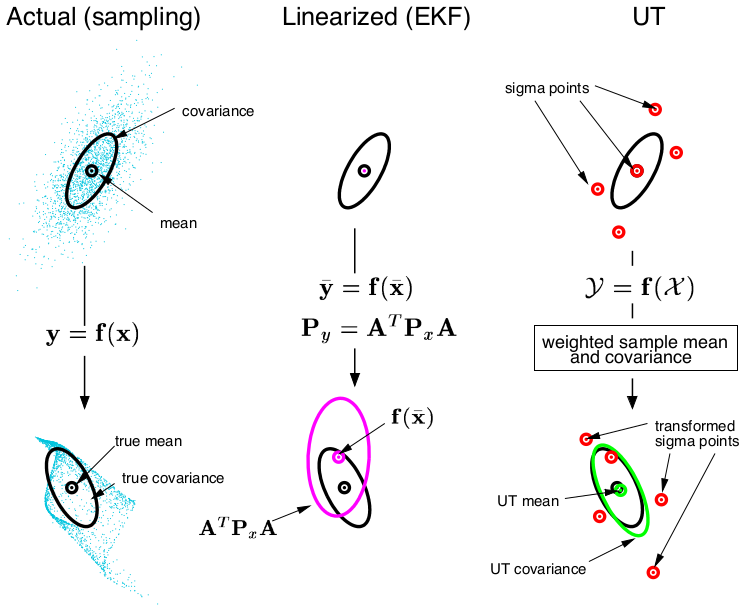
\includegraphics[width=10cm]{ukf}
  \caption{Example of the Unscented Transformation and its mean and covariance after the propagation step.
  (a) Monte Carlo sampling (b) Extended Kalman Filter (linearized) (c) Unscented Transformation (UKF). Taken from \cite{wan00}.}
  \label{fig:ukf}
\end{figure}

Fig. \ref{fig:ukf} illustrates three strategies where a \gls{pdf} is propagated through a non-linear function, where the first samples arbitrary points, the second performs a linearization of the function as in \gls{ekf}, and the third follows the above \gls{ut} strategy.

The full procedure for \gls{ukf} is identical to the original \gls{kf}, i.e. performs
a prediction step (as in Eq. \cref{eq:bg_apriori_estim,eq:bg_apriori_cov}), and
a correction step (as in Eq. \cref{eq:bg_innov,eq:bg_innov_cov,eq:bg_kf_gain,eq:bg_aposteriori_state_estim,eq:bg_aposteriori_cov_estim}) by applying the above sigma-points sampling and propagation step.

%%% Local Variables:
%%% mode: latex
%%% TeX-master: "../../main"
%%% End:



%%% Local Variables:
%%% mode: latex
%%% TeX-master: "../../main"
%%% End:
